\section*{Исходные данные}

\begin{itemize}
    \item Характеристическая скорость: $v_\t{хар} = 6430 \; \frac{\t{м}}{\t{с}}$
    \item Масса полезного груза: $M_\t{ПГ} = 2.2 \; \t{т}$
\end{itemize}

\section{Массовый расчет двухступенчатой ракеты}

Введем соотношение стартовых масс ступеней:
\begin{equation}
    \label{eq1}
    \lambda = \frac{M_{02}}{M_{01}}
\end{equation}
где $M_{01} = M_0$ --- стартовая масса ракеты.

Вторая ступень является полезным грузом для первой ступени:
\begin{equation}
    \label{eq2}
    M_\t{ПГ1} = M_{02}
\end{equation}

Тогда относительная масса полезного груза первой ступени равна
\begin{equation}
    \label{eq3}
    \mu_\t{ПГ1} = \frac{M_\t{ПГ1}}{M_{01}} = \frac{M_{02}}{M_{01}} = \lambda
\end{equation}

Тогда для второй ступени:
\begin{equation}
    \label{eq4}
    \mu_\t{ПГ2} = \frac{M_\t{ПГ}}{M_{02}} = \frac{M_\t{ПГ}}{\lambda M_{01}}
\end{equation}

Запишем весовые уравнения для двухступенчатой ракеты:
\begin{equation}
    \label{eq5}
    \begin{split}
        & \mu_\t{к1} = \frac{1}{1 + a_\t{ТО1}} \left( \lambda + a_{\t{ТО1}} + \frac{\gamma_\t{ДУ1}}{\nu_{01}} + \mu_\t{пр1} \right)
        \\
        & \mu_\t{к2} = \frac{1}{1 + a_\t{ТО2}} \left( \frac{M_\t{ПГ}}{\lambda M_{01}} + a_{\t{ТО2}} + \frac{\gamma_\t{ДУ2}}{\nu_\t{П2}} + \mu_\t{пр2} \right)
    \end{split}
\end{equation}

Весовые коэффициенты для топливной пары АТ + НДМГ принимают вид:
\begin{itemize}
    \item для первой ступени:
    \begin{equation}
        \label{eq6}
        \begin{cases}
            a_\t{ТО1} = 0.033 \left( 1 + 0.5\exp \left( -0.014 M_\t{Т1} \right) \right)
            \\
            \gamma_\t{ДУ1} = 0.012 \left( 1 + 1.0 \exp \left( -0.0009 P_\t{п1} \right) \right)
            \\
            \mu_\t{пр1} = 0.013 \left( 1 + 0.59 \exp \left( -0.0048 M_\t{01} \right) \right)
        \end{cases}
    \end{equation}
    \item для второй ступени:
    \begin{equation}
        \label{eq7}
        \begin{cases}
            a_\t{ТО2} = 0.033 \left( 1 + 0.5\exp \left( -0.014 M_\t{Т2} \right) \right)
            \\
            \gamma_\t{ДУ2} = 0.012 \left( 1 + 1.0 \exp \left( -0.0009 P_\t{п2} \right) \right)
            \\
            \displaystyle \mu_\t{пр2} = 0.013 \left( 1 + 0.59 \exp \left( -0.0048 M_\t{02} \right) \right) + \frac{0.25}{M_{02}}
        \end{cases}
    \end{equation}
\end{itemize}

где:
\begin{equation}
    \label{eq7.1}
    M_\t{Тi} = M_0 (1 - \mu_\t{кi})
\end{equation}
\begin{equation}
    \label{eq7.2}
    P_\t{пi} = \dot{m}_i \cdot J_\t{пi}
\end{equation}
\begin{equation}
    \label{eq7.3}
    \dot{m}_i = \frac{M_\t{Тi}}{t_i}
\end{equation}
\begin{equation}
    \label{eq7.4}
    t_i = \frac{J_\t{пi} \nu_i (1 - \mu_\t{кi})}{k_\t{п} g_0}
\end{equation}

Запишем формулу Циолковского для двухступенчатой ракеты:
\begin{equation}
    \label{eq8}
    v_\t{хар} = -J_\t{п1} \ln \mu_\t{к1} - J_\t{п2} \ln \mu_\t{к2}
\end{equation}

Примем следующие параметры:
\begin{itemize}
    \item Пустотный удельный импульс для топливной пары АТ + НДМГ: $\displaystyle J_\t{п1} = 3200 \; \frac{\t{м}}{\t{с}}$, $\displaystyle J_\t{п2} = \\ = J_\t{п1} + 100 \; \frac{\t{м}}{\t{с}} = 3300 \; \frac{\t{м}}{\t{с}}$
    \item Стартовая нагрузка на тягу: $\nu_{01} = 0.7$, $\nu_\t{п2} = 0.9$
    \item Коэффициент тяги в пустоте: $k_\t{п} = 1.15$
    \item Ускорение свободного падения $\displaystyle g_0 = 9.81 \; \frac{\t{м}}{\t{с}^2}$
\end{itemize}

Таким образом все параметры ракеты зависят только от стартовой массы ракеты $M_0 = M_{01}$ и распределения масс между ступенями $\displaystyle \lambda = \frac{M_{02}}{M_{01}}$. Искать параметры ракеты будем из расчета минимальной стартовой массы при условии равенства характеристической скорости рассчитанному ранее значению. Расчет будем проводить по следующему алгоритму:
\begin{enumerate}
    \item Задаемся первичными значениями $M_0$ и $\lambda$.
    \item Варьируем $\lambda$ при $M_0 = const$, находим $\lambda_{opt}$, при котором $v_\t{хар}$ принимает максимальное значение.
    \item Сравниваем заданную $v_\t{хар}$ с текущей и корректируем $M_0$.
\end{enumerate}

В результате расчетов получим:
\begin{equation}
    \label{eq9}
    M_0 = 28.014 \; \t{т}
\end{equation}
\begin{equation}
    \label{Eq10}
    \lambda_{opt} = 0.33
\end{equation}

\begin{figure}[H]
    \begin{center}
        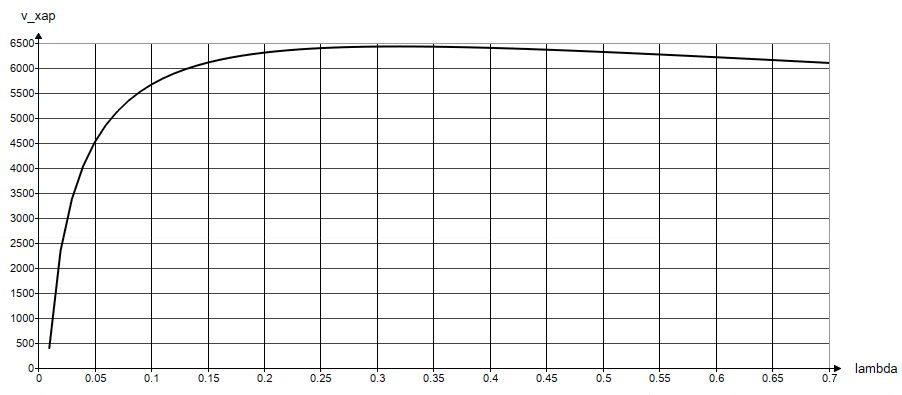
\includegraphics[width = 0.8\linewidth]{pic1.PNG}
        \caption{График распределения масс ступеней при $M_0 = 28.014 \; \t{т}$}
        \label{pic1}
    \end{center}
\end{figure}

Найдем весовые коэффициенты рассчитанной ракеты:
\begin{itemize}
    \item Первая ступень:
    \begin{equation}
        \label{eq10}
        \begin{cases}
            a_\t{ТО1} = 0.046
            \\
            \gamma_\t{ДУ1} = 0.019
            \\
            \mu_\t{пр1} = 0.02
            \\
            \mu_\t{к1} = 0.405
        \end{cases}
    \end{equation}
    \item Вторая ступень:
    \begin{equation}
        \label{eq11}
        \begin{cases}
            a_\t{ТО2} = 0.048
            \\
            \gamma_\t{ДУ2} = 0.023
            \\
            \mu_\t{пр2} = 0.047
            \\
            \mu_\t{к2} = 0.342
        \end{cases}
    \end{equation}
\end{itemize}

При этом характеристические скорости ступеней равны
\begin{equation}
    \label{eq11.1}
    v_\t{хар1} = -J_\t{п1} \ln \mu_\t{к1} = 2892.9 \; \frac{\t{м}}{\t{с}}
\end{equation}
\begin{equation}
    \label{eq11.2}
    v_\t{хар2} = -J_\t{п2} \ln \mu_\t{к2} = 3537.1 \; \frac{\t{м}}{\t{с}}
\end{equation}

\section{Сравнительный анализ результатов}

Стартовая масса одноступенчатой ракеты получилась равной
\begin{equation}
    \label{eq12}
    M_0 = 49.142 \; \t{т}
\end{equation}

Для двухступенчатой ракеты она равна
\begin{equation}
    \label{eq13}
    M_0 = 28.014 \; \t{т}
\end{equation}

Стартовые массы отличаются в 1,76 раза. Значительное отличие стартовых масс связано с большой дальностью $L = 3900 \; \t{км}$, поскольку проектировать одноступенчатые ракеты на такую дальность крайне невыгодно по массе.